\section{Security}

\subsection{Protocol}

A secure data transmission system always needs a cryptosystem. In this project, we use the RSA cryptosystem \cite{rsa} as it is fairly simple to implement.

Basically, the RSA algorithm generates a pair of distinct sequences called the public key and the private key. The receiver keeps the private key in secret whil publishing the public key to any sender. The sender encodes their message using the public key, which then can only be decrypted by anyone with the private key.

\begin{center}
    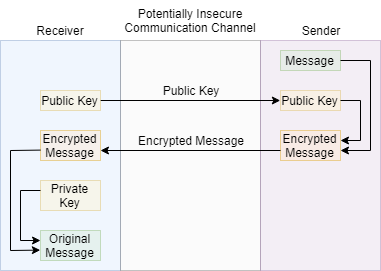
\includegraphics[]{images/rsa.png}
\end{center}

\subsection{Implementation}
We create a Python file named security.py and put all the functions for data encryption and decryption inside. These functions will later be imported to be uses in the MPI. 

\subsubsection{Key generation}

Basically, this function generates a public and a private key based on the RSA cryptosystem and then store them in two separate txt files.

\begin{minted}{python}
def gen_pair(save_dir: str='.'):
    key = RSA.generate(2048) # Generate 2048-bits key
    Path(save_dir).mkdir(exist_ok=True)
    private = key.export_key()
    private_path = Path(save_dir).joinpath('private.key.txt')
    with open(private_path, 'wb') as f:
        f.write(private)

    # Generate public key from a RSA key
    public = key.publickey().export_key()
    public_path = Path(save_dir).joinpath('public.key.txt')
    with open(public_path, 'wb') as f:
        f.write(public)
\end{minted}

This function imports the keys from txt files to be used in other functions.
\begin{minted}{python}
def import_key(private_key_file: str, public_key_file):
    private_key_file = Path(private_key_file)
    public_key_file = Path(public_key_file)

    private_key = RSA.import_key(open(private_key_file, 'r').read())
    public_key = RSA.import_key(open(public_key_file, 'r').read())
    return private_key, public_key

\end{minted}

\subsubsection{Encryption}

\begin{center}
    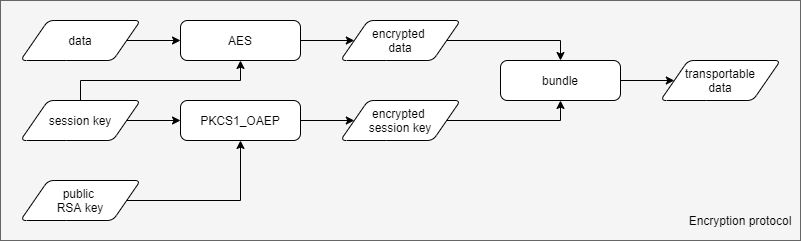
\includegraphics[scale=0.5]{images/encryption_protocol.png}
\end{center}

This function encodes a string of data into a bundle of bytes which is transportable. It takes three arguments:
\begin{itemize}
    \item A string of data that needs to be encrypted
    \item previously generated RSA public key
    \item a randomly generated session key
\end{itemize}

\begin{minted}{python}
def encode_encrypt(data: str, public_key: RSA.RsaKey):
    encoded_data = data.encode()
    session_key = get_random_bytes(16)

    cipher_RSA = PKCS1_OAEP.new(key=public_key)
    encrypted_session_key = cipher_RSA.encrypt(session_key)

    cipher_AES = AES.new(session_key, AES.MODE_EAX)
    encrypted_data, tag = cipher_AES.encrypt_and_digest(encoded_data)

    bundle = (encrypted_session_key, cipher_AES.nonce, tag, encrypted_data)
    return dumps(bundle)

\end{minted}

\subsubsection{Decryption}

\begin{center}
    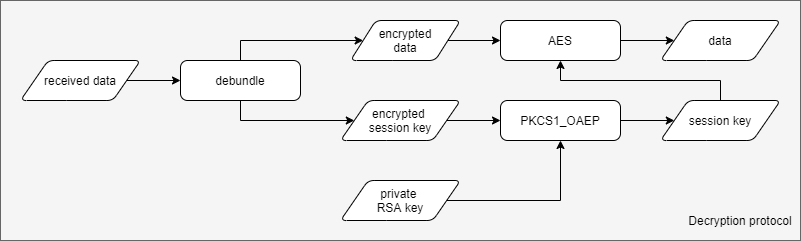
\includegraphics[scale=0.5]{images/decryption_protocol.png}
\end{center}

This function turns the received data into a bundle of bytes that contain the encrypted data and the encrypted session key. Using these two and the previously generated RSA private key, it returns the decrypted data.

\begin{minted}{python}
def decrypt_decode(bundle: bytes, private_key: RSA.RsaKey):
    session_key, nonce, tag, encrypted_data = loads(bundle)

    cipher_RSA = PKCS1_OAEP.new(key=private_key)
    session_key = cipher_RSA.decrypt(session_key)

    cipher_AES = AES.new(session_key, AES.MODE_EAX, nonce)
    encoded_data = cipher_AES.decrypt_and_verify(encrypted_data, tag)

    return encoded_data.decode()

\end{minted}